\chapter{Descrição do Processo}
\label{chap:descricaoprocesso}

Este capítulo apresenta o sistema de propulsão do automodelo utilizado como objeto de estudo
e discute as abordagens de instrumentação consideradas para a caracterização de sua dinâmica.
Para cada abordagem, são apresentados o princípio de funcionamento, a proposta de controle em
malha fechada, as vantagens e as limitações, de modo a fundamentar as decisões do projeto.

\section{O Automodelo e seu Sistema de Propulsão}
\label{sec:automodelo}

O automodelo Kyosho Mad Force Kruiser 2.0 VE é equipado com um motor brushless Orion Ori28188, cuja
constante de velocidade é de \(2100\,\mathrm{rpm/V}\) --- rotações por minuto por volt aplicado,
em condições próximas à operação sem carga mecânica significativa.
Esse motor é constituído por um estator, componente fixo com núcleo ferromagnético envolvido por
enrolamentos de fio de cobre, e por um rotor, componente móvel com ímãs permanentes fixados na
carcaça. No rotor, os ímãs permanentes produzem campo magnético próprio em razão das
propriedades do material; no estator, a corrente elétrica que percorre os enrolamentos gera um
campo eletromagnético. A interação entre esses dois campos produz
o torque responsável pela rotação do eixo, como ilustrado na Figura~\ref{fig:motorbrushless}.

\begin{figure}[htb]
\centering
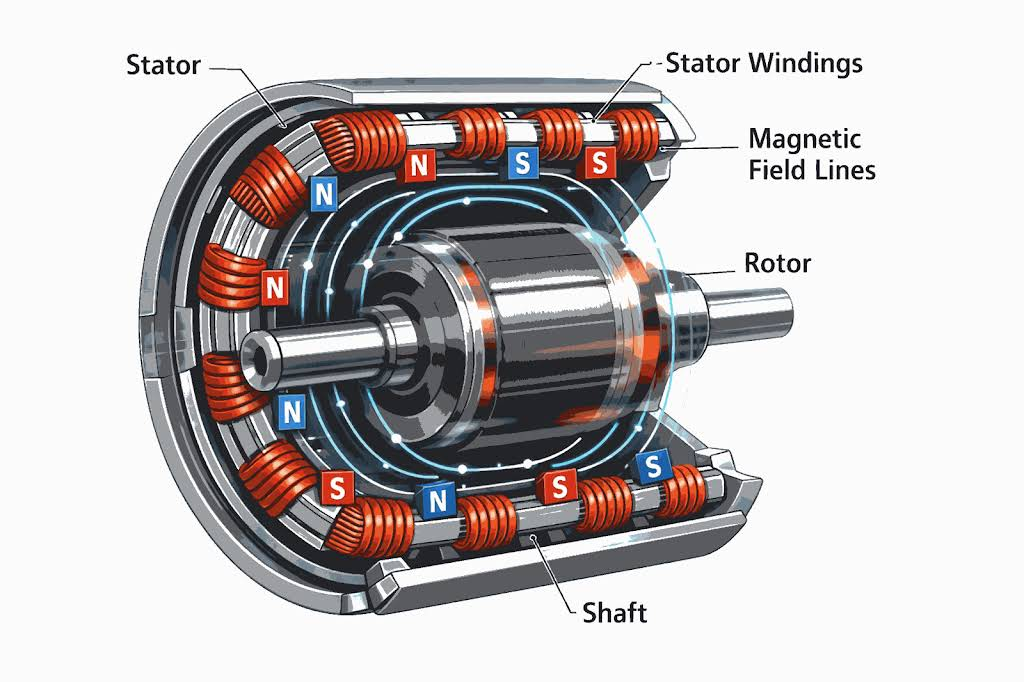
\includegraphics[width=0.8\textwidth]{DescricaoProcesso/Figuras/motor_explode.jpeg}
\caption{Visão explodida de um motor brushless --- o campo magnético produzido pelo estator interage com os ímãs permanentes do rotor, gerando torque.}
\label{fig:motorbrushless}
\footnotesize{Fonte: DIGI Electronics (s.d.). Disponível em: \url{https://www.digi-electronics.com/en/blogs/stator-vs-rotor-construction-functions-and-maintenance/518.html}.}
\end{figure}

A continuidade desse movimento depende da comutação eletrônica, processo pelo qual a alimentação das três fases
do motor é alternada em uma sequência que modifica continuamente a orientação do campo magnético resultante do estator,
produzindo um campo girante. Essa função é realizada pelo Controlador Eletrônico de Velocidade (\emph{Electronic
Speed Controller} --- ESC) Orion Vortex R8, que recebe do receptor de rádio o comando de aceleração e controla a energia
elétrica transferida da bateria para os enrolamentos. Como o motor é do tipo \emph{sensorless}, o ESC estima sua
posição a partir da força contraeletromotriz (\emph{back-EMF}) --- a tensão induzida nos enrolamentos pela rotação dos
ímãs permanentes do rotor. Para isso, uma das fases permanece temporariamente sem alimentação durante a comutação,
permitindo ao controlador detectar os cruzamentos por zero dessa tensão e estimar os instantes adequados para a
próxima etapa. Dessa forma, o ESC mantém o campo do estator sincronizado com o movimento do rotor, possibilitando
a conversão contínua da energia elétrica em energia mecânica.

Segundo o manual do fabricante, o ESC suporta corrente
contínua de até 120 A e corrente de pico de até 760 A.
A alimentação do sistema é realizada por uma bateria de polímero de lítio (LiPo) de duas células, com tensão nominal de 7,4 V,
capacidade de 5200 mAh e taxa de descarga de 60C. Ao longo do trabalho, também são empregadas baterias
preexistentes, com anos de uso, cujo efeito sobre os ensaios será analisado. O comando de aceleração aplicado ao ESC 
pode ter duas origens, selecionadas por uma chave de comutação: o sinal
PWM (\emph{Pulse Width Modulation} --- modulação por largura de pulso, na qual a largura dos pulsos codifica o comando)
proveniente do controle remoto, por meio do receptor de rádio, ou o sinal
gerado por uma Raspberry Pi embarcada no veículo, que possui bateria própria e conversor
\emph{step-down} para alimentação em 5 V.


\section{Situação Atual e Estado da Arte}
\label{sec:estadoarte}

Para atender os objetivos, podem ser consideradas
diferentes alternativas de medição, e a escolha da mais adequada entre elas depende de fatores
como precisão, complexidade de implementação, custo e adequação às condições experimentais.
Nesse contexto, as subseções a seguir apresentam o princípio de funcionamento de cada técnica,
discutem sua aplicabilidade na caracterização do sistema e fundamentam a opção adotada.

\subsection{Sensor Inercial (IMU)}
\label{sec:imu}

A primeira lei de Newton estabelece que um corpo livre de forças externas tende a manter seu
estado de movimento --- repouso ou deslocamento retilíneo e uniforme ---, de modo que qualquer
mudança na velocidade, em magnitude ou em direção, exige a ação de uma força resultante não nula.
Essa resistência que a matéria oferece às mudanças de seu estado de movimento é denominada
inércia, e ela constitui o princípio físico explorado pela instrumentação inercial. Na
translação, a medida da inércia de um corpo é sua massa: quanto maior a massa, maior a força
necessária para produzir a mesma variação de velocidade no mesmo intervalo de tempo. Na rotação,
o papel análogo é desempenhado pelo momento de inércia, que quantifica a resistência às mudanças
de velocidade angular e depende tanto da massa quanto de sua distribuição em relação ao eixo de
giro. Assim, a inércia não é uma propriedade acessória do movimento, mas a grandeza que todo
sensor inercial converte em medida.

A Unidade de Medição Inercial (\emph{Inertial Measurement Unit} --- IMU) é um instrumento que
mede o movimento próprio do corpo ao qual está fixado, sem referência a nenhum elemento externo,
daí o adjetivo \emph{inercial}. Seu princípio de funcionamento consiste em explorar justamente a
resistência descrita acima: quando a carcaça do sensor é acelerada junto com o veículo, um corpo
de prova interno, em razão de sua inércia, tende a permanecer em seu estado anterior e, com isso,
se desloca em relação à carcaça. Medindo esse deslocamento relativo --- a reação do corpo de
prova à aceleração imposta ---, o sensor estima a aceleração a que o conjunto está sujeito, sem
contato com o solo, sem marcas externas e sem sinais de rádio. Dessa forma, a IMU reúne, em um
único dispositivo, um acelerômetro e um giroscópio, que realizam essa medião para as
translações e para as rotações, respectivamente.

No acelerômetro de tecnologia MEMS (\emph{Micro-Electro-Mechanical Systems} --- sistemas
microeletromecânicos), o corpo de prova é uma massa microfabricada, suspensa por molas flexíveis
a uma estrutura que se move solidariamente à carcaça. Quando o veículo acelera, a carcaça e a
estrutura acompanham o movimento imediatamente, ao passo que a massa de prova, atrasada pela
inércia, resiste à variação e se desloca relativamente à estrutura até que as molas restabeleçam
o equilíbrio. Esse deslocamento relativo é tipicamente medido pela variação de capacitância entre
placas microfabricadas que se aproximam ou se afastam, e, em regime, o equilíbrio entre a força
de inércia que age sobre a massa de prova e a força elástica das molas satisfaz

\begin{equation}\label{eq:acelerometro}
m_p\,a = k_m\,x,
\end{equation}

em que $m_p$ é a massa de prova, $a$ a aceleração da carcaça, $k_m$ a constante elástica das
molas e $x$ o deslocamento relativo, de modo que $a = (k_m/m_p)\,x$ e a aceleração se obtém
diretamente do deslocamento medido. Cabe uma ressalva importante: o acelerômetro não distingue,
em sua leitura bruta, a aceleração do movimento da aceleração da gravidade, uma vez que a
aceleração própria medida inclui a componente correspondente à força de apoio que sustenta o
sensor. Para separar a gravidade da aceleração efetiva do veículo, é necessário estimar
continuamente a orientação do sensor --- sua atitude ---, o que normalmente é feito combinando-se
as leituras do acelerômetro e do giroscópio em um filtro de fusão.

O giroscópio MEMS, por sua vez, mede a velocidade angular recorrendo ao efeito Coriolis: uma
estrutura oscilante interna, mantida em vibração por atuadores eletrostáticos, ao sofrer rotação
do conjunto, desenvolve uma força perpendicular à direção da oscilação e proporcional à
velocidade angular imposta. Essa força desloca lateralmente a estrutura vibrante, e o
deslocamento, medido pelas mesmas técnicas capacitivas do acelerômetro, fornece a taxa de
rotação em cada eixo, usualmente em graus por segundo (°/s). A principal limitação clássica do
giroscópio é a deriva (\emph{drift}): pequenos erros sistemáticos de \emph{bias} presentes em
cada leitura, quando integrados ao longo do tempo para se obter o ângulo, crescem sem limite e
fazem a estimativa de orientação se afastar progressivamente da orientação real.

Essas duas medições se relacionam com o veículo de forma direta. A aceleração longitudinal
integrada uma vez no tempo fornece a velocidade, e integrada duas vezes fornece a posição;
na prática, contudo, a integração pura é inviável em poucos segundos, pois o \emph{drift} do
giroscópio e o \emph{bias} do acelerômetro se acumulam exatamente como na estimativa de
orientação. Por isso, a velocidade obtida de uma IMU em aplicações reais é sempre resultado de
uma fusão com outras fontes --- um receptor GPS ou um encoder de roda ---, que fornecem
referências externas capazes de limitar o crescimento do erro. Além disso, a IMU mede a
dinâmica do chassi, e não do \emph{powertrain}: a aceleração que ela capta é o efeito líquido
da ação propulsora já descontadas as resistências, de modo que nem o torque do motor nem a
força de tração são acessíveis diretamente em sua leitura. O torque do motor se transforma em
força de tração na roda, que deve vencer as forças resistivas ao movimento para resultar na
aceleração do veículo; aplicando a segunda lei de Newton:

\begin{equation}\label{eq:newton}
m\,a = F_{\text{tração}} - F_{\text{resistivos}},
\end{equation}

em que $m$ é a massa do veículo e $F_{\text{resistivos}}$ reúne as contribuições do atrito de rolamento
e do arrasto aerodinâmico. Na roda, a força de tração é dada por $F_{\text{tração}} = T_\mathrm{roda}/r$, sendo $r$ o
raio efetivo da roda, e o torque nas rodas é o torque do motor multiplicado pela redução $i$ e
pelo rendimento $\eta$ da transmissão,

\begin{equation}\label{eq:transmissao}
T_\mathrm{roda} = i\,\eta\,T_{\text{motor}}.
\end{equation}

Combinando as Equações \eqref{eq:newton} e \eqref{eq:transmissao}, o torque do motor poderia ser
estimado a partir da aceleração medida:

\begin{equation}\label{eq:torque_motor}
T_{\text{motor}} = \frac{r\,(m\,a + F_{\text{resistivos}})}{i\,\eta}.
\end{equation}

Essa estimativa, contudo, exige que se desfaça toda a cadeia de transformações que vai da causa ao
efeito: cada passo da operação inversa requer um parâmetro que a IMU não mede, como a massa $m$,
as resistências $F_{\text{resistivos}}$, o raio da roda $r$ e o rendimento $\eta$. A IMU, portanto, informa
como o veículo responde, mas não quanto o propulsor efetivamente produz.

Na implementação prática, o sensor considerado foi o MPU-6050, que reúne acelerômetro e
giroscópio triaxiais em um único circuito integrado. O microcontrolador o lê por meio do
barramento I$^2$C, que emprega apenas dois sinais --- SDA (\emph{Serial Data}), por onde transitam
as informações, e SCL (\emph{Serial Clock}), que sincroniza a troca ---, além da alimentação.
Nesse barramento, cada dispositivo é reconhecido por um endereço fixo, o que permite
compartilhar os mesmos dois fios com outros sensores. A Figura~\ref{fig:imu_i2c} ilustra a
ligação com um Arduino: quatro fios conectam a alimentação ($V_{CC}$ e GND) e os dois sinais do
barramento. Em malha fechada, o controlador executado no microcontrolador compararia a
velocidade estimada à referência e enviaria o comando de aceleração ao ESC por um sinal PWM,
sem acionar o motor diretamente.

\begin{figure}[htb]
\centering
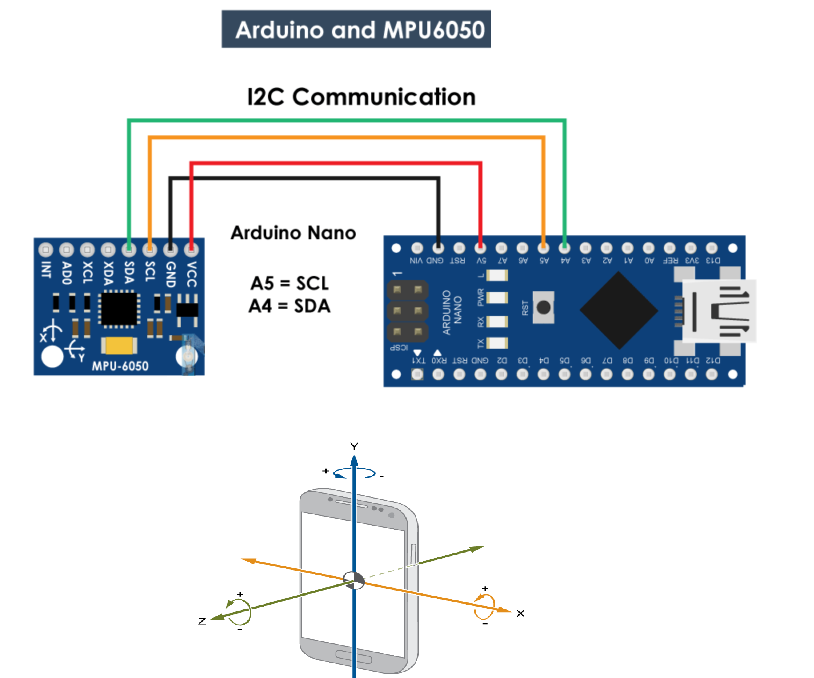
\includegraphics[width=0.75\textwidth]{DescricaoProcesso/Figuras/imu_mpu6050_i2c.png}
\caption{Ligação do MPU-6050 a um microcontrolador Arduino via I$^2$C: quatro fios conectam a alimentação e os sinais SDA e SCL do barramento.}
\label{fig:imu_i2c}
\footnotesize{Fonte: RudraNarayanG, via Instructables (s.d.). Disponível em: \url{https://www.instructables.com/Accelerometer-MPU-6050-Communication-With-AVR-MCU/}.}
\end{figure}

Quanto à adequação ao objetivo deste trabalho, as vantagens da IMU são o desempenho sem contato
mecânico adicional, o formato compacto e embutido, o baixo custo e a interface digital simples.
As desvantagens são o \emph{drift} que inviabiliza a integração pura, a sensibilidade à vibração
intensa do veículo de pequena escala e, sobretudo, o fato de não medir diretamente nenhuma
grandeza da cadeia elétrica ou de torque do propulsor. Uma vez que o objetivo do projeto é
estimar torque e tração a partir da corrente elétrica, a IMU viabilizaria apenas a
caracterização dinâmica longitudinal do veículo --- a relação entre comando e velocidade ---,
configurando alternativa para trabalho futuro, e não o sensor adequado ao propósito central da
caracterização proposta.

\subsection{Sensor Magnético de Efeito Hall SS41F/41G}
\label{sec:ss41f}

O SS41F/41G é um sensor digital de efeito Hall do tipo bipolar, cuja
saída assume nível alto na presença do polo norte de um ímã e nível baixo na presença do polo sul. Quando um anel
magnetizado --- um ímã de ferrita com polos alternados ao longo da circunferência --- gira rigidamente
acoplado à roda ou ao eixo, o sensor produz $N$ transições digitais por revolução, sendo $N$ o número de
alternâncias de polos. Esse é o princípio dos encoders de roda usualmente empregados em robótica,
nos quais o microcontrolador conta as transições em uma janela de tempo para estimar a rotação.

Com $c$ pulsos contados em uma janela de duração $T_j$, a velocidade angular do eixo que carrega o
anel é $\omega = 2\pi c/(N T_j)$. Com o anel no eixo do motor, a contagem fornece diretamente a
velocidade $\omega_m$; com ele na roda, fornece $\omega_\mathrm{roda}$, que se converte em
$\omega_m$ pela redução $i$ da transmissão.

A estimativa de torque a partir da velocidade, contudo, requer a dinâmica rotacional do conjunto. Com
momento de inércia $J$ refletido no eixo do motor, coeficiente de atrito viscoso $B$ e torque de
carga $T_L$, a segunda lei de Newton para a rotação resulta em
\begin{equation}\label{eq:dinamica_rotacional}
T_{\text{motor}} = J\,\frac{d\omega_m}{dt} + B\,\omega_m + T_L.
\end{equation}

O torque depende, nesse caso, da derivada da velocidade medida e de três parâmetros, $J$, $B$ e $T_L$,
que precisariam ser identificados separadamente. Há, ainda, um limite de resolução inerente ao
método, pois, em baixas rotações, poucos pulsos são contados e a estimativa se
torna progressivamente mais grosseira. A derivada exigida pela Equação
\eqref{eq:dinamica_rotacional} amplifica esse ruído de quantização, tornando a estimativa de
torque sensível à resolução do sensor e, em última instância, ao número de polos do anel.

Em malha fechada, a velocidade medida pode realimentar diretamente um controlador
de velocidade, sem nenhum modelo de torque, da mesma forma que a velocidade estimada pela IMU.
Motores brushless com sensores Hall integrados já são controlados dessa maneira, com os mesmos
sinais servindo à comutação e à realimentação.

Em síntese, as vantagens e desvantagens do SS41F/41G são as seguintes.

\begin{enumerate}
    \item Vantagens: baixo custo, robustez mecânica e velocidade de comutação superior a 100 kHz, com interface digital simples, compatível com a leitura por interrupção em microcontroladores comuns; e fornece a velocidade por contagem direta dos pulsos.
    \item Desvantagens: gera apenas pulsos associados à posição angular, sem informação sobre corrente elétrica ou torque; a estimativa de torque só é possível após a determinação de $J$, $B$ e $T_L$, conforme a Equação \eqref{eq:dinamica_rotacional}; e a instalação demanda alinhamento mecânico preciso entre o sensor e o anel, pois desalinhamentos produzem pulsos assimétricos que distorcem a medida.
\end{enumerate}

\subsection{Shunt Resistivo e Amplificador de Instrumentação (INA240)}
\label{sec:ina240}

No arranjo com shunt resistivo, um resistor de baixa resistência $R_s$ é inserido em série com o
caminho da corrente. Pela Lei de Ohm, a queda de tensão sobre ele é

\begin{equation}\label{eq:shunt_ohm}
V_s = R_s\,I.
\end{equation}

Essa tensão, tipicamente da ordem de milivolts, é amplificada pelo circuito integrado INA240, cuja
saída, referenciada a uma tensão de polarização $V_\mathrm{bias}$, é
\begin{equation}\label{eq:shunt_ganho}
V_\mathrm{out} = G\,R_s\,I + V_\mathrm{bias},
\end{equation}
em que $G$ é o ganho fixo do amplificador.

% TODO: inserir figura do INA240 (Relatório 1)

O componente possui largura de banda de 400 kHz e
rejeição reforçada a transientes de modo comum --- variações rápidas e simultâneas da tensão nos
dois terminais de entrada, justamente as produzidas pelo chaveamento de um ESC. Em altas
frequências, a indutância parasita do resistor faz com que a tensão deixe de ser proporcional à
corrente instantânea, distorcendo a leitura durante o chaveamento.

A dissipação de potência no resistor cresce com o quadrado da corrente; com isso, sob correntes
elevadas, o shunt aquece e consome parte da energia destinada ao motor. Observa-se, ainda, que instalado na alimentação do ESC mede a corrente média de entrada, e não a corrente de
fase do motor, que é chaveada pelo PWM. Na aproximação usual, a corrente de entrada se
relaciona à de fase pela razão cíclica $D$ do chaveamento --- a fração do período em que o PWM
permanece ligado:

\begin{equation}\label{eq:corrente_bateria}
\bar{I}_\mathrm{bat} \approx D\,I_\mathrm{fase}.
\end{equation}

Consequentemente, a leitura precisa ser interpretada considerando o ciclo de trabalho vigente. Essa ressalva
se aplica igualmente a qualquer sensor instalado no ramo de alimentação, como se verá adiante.

Em síntese, as vantagens e desvantagens do arranjo com shunt e INA240 são as seguintes.

\begin{enumerate}
    \item Vantagens: proporciona uma medida direta da corrente, com boa linearidade e ampla largura de banda a baixo custo.
    \item Desvantagens: dissipação de potência sob correntes elevadas, distorção da leitura em alta frequência decorrente da indutância parasita do resistor e ausência de isolamento galvânico --- contato elétrico direto entre o circuito de medição e o de potência.
\end{enumerate}

Dessa forma, o arranjo com shunt reúne banda e linearidade adequadas à medição, mas a ausência de
isolamento galvânico e a dissipação crescente com o quadrado da corrente afastam-no da montagem de
bancada adotada neste trabalho, na qual o circuito de medição permanece próximo ao computador de bordo.

\subsection{Sensor de Efeito Hall Linear (ACS758/ACS712)}
\label{sec:acshall}

Os sensores de efeito Hall lineares, como as famílias ACS758 e ACS712, medem a corrente de forma
indireta e sem contato elétrico com o circuito de potência. Seu princípio é o efeito Hall: quando
uma corrente atravessa um condutor exposto a um campo magnético perpendicular, as cargas em
movimento sofrem uma deflexão lateral, gerando uma tensão transversal proporcional ao campo. No
sensor, a corrente a ser medida percorre um condutor interno e cria, em seu entorno, um campo
magnético; elementos Hall próximos a esse condutor detectam o campo e a eletrônica integrada
converte a tensão gerada em uma tensão de saída proporcional à corrente. Na variante bidirecional
do ACS758, a saída é

\begin{equation}\label{eq:acs_saida}
V_\mathrm{out} = \frac{V_{CC}}{2} + S\,I,
\end{equation}
em que $S$ é a sensibilidade, em V/A, e $V_{CC}/2$ é a tensão de repouso, correspondente a
corrente nula. A corrente é recuperada por
\begin{equation}\label{eq:acs_corrente}
I = \frac{V_\mathrm{out} - V_{CC}/2}{S}.
\end{equation}

Esse tipo de sensor já foi empregado em um motor brushless do tipo \emph{hub}, relacionando a
corrente de fase medida à força de tração, à potência e à eficiência de um veículo elétrico de
baixa potência. Também já foi aplicado em dinamômetros de baixo custo voltados a
motores brushless de uso amador, acoplado a células de carga, o que evidencia a
viabilidade desse sensor em montagens de bancada sem equipamentos dedicados de laboratório.

A sensibilidade é definida pela variante escolhida, que determina também a faixa de medição. Na
família ACS758 bidirecional, as variantes de ±50 A, ±100 A, ±150 A e ±200 A apresentam,
com alimentação nominal de 5 V, sensibilidades típicas de 40 mV/A, 20 mV/A, 13,3 mV/A e 10 mV/A,
respectivamente. Como a saída é ratiométrica --- isto é, ambas as grandezas se ajustam
proporcionalmente à alimentação ---, a operação a 3,3 V adotada neste trabalho reduz a
sensibilidade da variante de ±200 A para aproximadamente 6,6 mV/A. Em qualquer alimentação, uma
faixa maior implica menor sensibilidade e, consequentemente, menor resolução para a mesma
conversão. Essa resolução é limitada pela conversão
analógico-digital de $n$ bits e por sua tensão de referência $V_\mathrm{ref}$ --- o menor degrau
de tensão que o conversor distingue:
\begin{equation}\label{eq:acs_resolucao}
\Delta I = \frac{V_\mathrm{ref}}{2^{n}\,S}.
\end{equation}
Com conversor de 12 bits e referência de 3,3 V, a variante de ±200 A resulta, na prática deste
trabalho, em resolução de cerca de 122 mA. Para correntes de dezenas de ampères, essa resolução é
suficiente, embora limite a medida de variações pequenas em torno do repouso.

A folha de dados (\emph{datasheet}) especifica tempo de resposta de 4 µs e largura de banda
interna de 120 kHz, valor bem superior à faixa de 8 kHz a 16 kHz de chaveamento
típica de ESCs \emph{sensorless}. Logo, o sensor dispõe de margem para acompanhar as
variações de corrente impostas pela comutação, sem subamostrá-las.

O isolamento galvânico dispensa modificação do circuito de potência além da inserção em série do
próprio sensor, e não introduz dissipação adicional significativa. Como limitações, ele
permanece sujeito a ruído eletromagnético proveniente do chaveamento do ESC, o que pode exigir
filtragem do sinal antes da aquisição. A faixa máxima das variantes, de ±200 A, é inferior ao
pico de 760 A especificado para o ESC, o que deixa os picos extremos de corrente fora da
faixa de medição. A operação a 3,3 V desloca os valores nominais de repouso e de sensibilidade,
devendo ser tratada como condição de calibração experimental própria, o que é feito no Capítulo 3.
Por fim, a relação entre corrente e torque pode deixar de ser aproximadamente linear em correntes
elevadas, exigindo calibração experimental adicional, também retomada naquele capítulo.

Em síntese, as vantagens e desvantagens do ACS758 são as seguintes.

\begin{enumerate}
    \item Vantagens: isolamento galvânico, sem dissipação adicional significativa e com banda suficiente para o chaveamento do ESC.
    \item Desvantagens: resolução inferior à do shunt para a mesma faixa, faixa máxima inferior ao pico do ESC, sensibilidade dependente da alimentação e sensibilidade a ruído eletromagnético.
\end{enumerate}

Assim, entre os sensores de corrente avaliados, o ACS758 reúne o melhor compromisso entre
isolamento galvânico, dissipação, faixa de medição e banda para as correntes e frequências deste
sistema, sendo o sensor adotado neste trabalho para a medição da corrente de bateria.

\subsection{Síntese Comparativa}
\label{sec:sintese}

As quatro abordagens medem grandezas distintas, e cada uma se associa ao torque por um caminho
próprio. A IMU mede a aceleração linear e a velocidade angular do chassi, o SS41F/41G mede a
velocidade angular de uma roda ou do eixo por pulsos, e o shunt e o sensor Hall linear medem a
corrente elétrica por princípios físicos distintos.

Para os sensores de corrente, a relação entre o torque eletromagnético e a corrente é dada pela
constante de torque $K_t$,
\begin{equation}\label{eq:torque_corrente}
T_{\text{motor}} = K_t\,I.
\end{equation}
Essa constante traduz, num único número, a capacidade do motor de converter corrente em torque.
Em motores brushless, ela é numericamente igual à constante de
força contraeletromotriz, em V·s/rad --- um reflexo da conservação da energia: a mesma constante
que converte corrente em torque converte rotação em tensão. A constante de velocidade $K_v$, dada
em rpm/V, se
relaciona a ambas por
\begin{equation}\label{eq:ke_kv}
K_t = K_e = \frac{60}{2\pi\,K_v} \approx \frac{9{,}55}{K_v},
\end{equation}
em que o fator 9,55 é o valor numérico de $60/(2\pi)$, que converte rotações por minuto em
radianos por segundo. Para o motor do automodelo, com $K_v = 2100$ rpm/V, obtém-se
$K_t \approx 4{,}5$ mN$\cdot$m/A. Com a redução $i \approx 11{,}5$ e desprezando, em primeira
análise, as perdas da transmissão, o torque nas rodas é
\begin{equation}\label{eq:torque_roda_corrente}
T_\mathrm{roda} = i\,K_t\,I \approx 52\ \mathrm{mN\cdot m/A}\cdot I.
\end{equation}
Essa é uma estimativa idealizada, válida apenas na faixa em que a relação entre corrente e torque
permanece aproximadamente linear, a qual a caracterização experimental deste trabalho determina.

A diferença entre as abordagens está, sobretudo, na cadeia de dependências até o torque. A IMU e o
SS41F/41G exigem a identificação prévia de parâmetros mecânicos ($m$, $F_{\text{resistivos}}$, $J$, $B$ e $T_L$). A corrente elétrica dispensa esses parâmetros, mas sua relação com o torque
depende da posição do sensor no circuito, conforme a Equação \eqref{eq:corrente_bateria}.

Entre os sensores de corrente, a escolha envolve o compromisso entre isolamento elétrico, dissipação
de potência, faixa de medição e desempenho dinâmico sob chaveamento. O shunt oferece maior largura
de banda a menor custo, mas não é isolado e dissipa potência. O sensor Hall é isolado e praticamente
não dissipa potência, mas tem faixa limitada e demanda atenção ao ruído e à calibração da alimentação.

Existe ainda uma alternativa que dispensa qualquer sensor de corrente. Nela, o torque de motores
brushless usados em multirrotores é estimado a partir apenas da tensão de
alimentação, do comando de aceleração e da velocidade de rotação, ajustando-se um modelo de
quatro parâmetros ao conjunto motor, ESC e hélice. Essa abordagem evita a instrumentação elétrica
do sistema de propulsão, mas o modelo precisa ser recalibrado para cada motor, ESC e carga
mecânica utilizados. Sua viabilidade para o automodelo depende, desse modo, da variabilidade entre
configurações de transmissão e regimes de carga, cuja investigação fica como proposta de
continuidade deste trabalho.

Assim, a corrente elétrica é a grandeza com a cadeia de dependências mais curta até o torque, e,
entre os sensores de corrente, o Hall linear oferece o melhor equilíbrio entre isolamento, custo e
simplicidade de montagem para as correntes e frequências deste sistema. O sensor magnético
SS41F/41G, embora não empregado na caracterização proposta, viabiliza um ensaio em vazio com
rotação --- com anel magnetizado no eixo e veículo suspenso --- que permitiria medir a constante de
velocidade real do motor e a dinâmica entre comando e velocidade angular, configurando proposta de
continuidade. A forma de combinar o ACS758 a uma medição direta do esforço de tração constitui a
proposta de instrumentação deste trabalho, apresentada na Seção~\ref{sec:proposta}.

\section{Proposta do Projeto}
\label{sec:proposta}

Com base na comparação apresentada na Seção~\ref{sec:sintese}, este trabalho propõe a
caracterização do sistema de propulsão do automodelo por meio de sua curva característica torque
versus corrente. Para tanto, emprega-se uma instrumentação combinada: o sensor de efeito Hall
linear ACS758 de ±200 A, instalado no ramo de alimentação do ESC, fornece a corrente elétrica
consumida; uma balança digital de gancho, instalada na linha de tração do veículo, mede a
força desenvolvida.

A medição da força de tração segue a configuração do ensaio de \emph{drawbar pull} --- ensaio de
tração com o veículo ancorado ---, empregado na caracterização de veículos planetários, de robôs
terrestres de pequeno porte e de protótipos de baixo custo que substituem a célula de carga por
balanças digitais de gancho. Nessa configuração, o
veículo é ancorado e a balança, instalada na linha de tração, mede a própria força desenvolvida,
e o torque na roda é obtido diretamente por $T_\mathrm{roda} = F_{\text{tração}}\,r$, com um único
parâmetro geométrico. A escolha da balança digital de mala em lugar de uma célula de carga
dedicada segue o mesmo princípio de baixo custo já adotado na seleção do sensor de corrente.
Automodelos instrumentados têm sido empregados em trabalhos recentes, tanto em ensaios dinâmicos
para o ensino de engenharia
quantum em plataformas de aquisição de dados
off-road na mesma escala 1/8 do veículo utilizado neste trabalho.
Nesses casos, contudo, a instrumentação visa a dinâmica de movimento, e não o ensaio de tração
estacionário com medição simultânea de força e corrente proposto aqui.

O ensaio é conduzido com o veículo acrescido de dois halteres de 1 kg fixados próximo ao centro de
massa, totalizando 7,14 kg, condição adotada para elevar a aderência disponível entre pneus e
piso. A massa não entra no equilíbrio estático da medição --- na configuração ancorada, a força
registrada na balança iguala a tração desenvolvida, independentemente da massa do veículo ---, mas
define o limite de patinagem: a tração máxima transferida cresce com a carga normal sobre as rodas
motrizes, e a especificação da massa do veículo integra a condição de ensaio em procedimentos de
referência para ensaios de tração de veículos \emph{off-road}. A curva característica obtida é,
portanto, uma propriedade do conjunto propulsor, referida a essa condição de carregamento.

A combinação das duas medições permite construir a curva característica torque versus corrente
ponto a ponto, relacionando o esforço mecânico produzido ao esforço elétrico consumido. Para além
da característica estática, o projeto contempla a dinâmica do caminho de comando até a corrente,
uma vez que é sobre essa dinâmica que a malha de controle atua. Dois ensaios complementares
fornecem os dois modelos.

O primeiro, denominado ensaio dinâmico, dispensa a leitura da balança --- daí também ser chamado
ensaio cego --- e aplica degraus de comando na região de aderência do pneu, entre 100° e 110°,
com a corrente de bateria amostrada a 100 Hz por firmware dedicado. Com o comando normalizado
$u = (\theta - 95^\circ)/85^\circ$, que mapeia o neutro ($95^\circ$) em $u = 0$ e o máximo
($180^\circ$) em $u = 1$, a identificação por resposta ao degrau resulta na função de
transferência

\begin{equation}\label{eq:ft_ui}
G_1(s) = \frac{I(s)}{u(s)} = \frac{120\,e^{-\theta_a s}}{1{,}8\,s + 1},
\end{equation}

em que $120$ A/u é o ganho estático, $1{,}8$ s é a constante de tempo dominante --- atribuída ao
escalonamento interno do ESC --- e $\theta_a < 0{,}1$ s é o atraso, inferior à resolução temporal do
ensaio.

O segundo é o ensaio de tração estática, no qual o protocolo de degraus é repetido com o veículo
ancorado e a força anotada na balança durante o platô de cada degrau. A corrente medida no ramo de
alimentação é a corrente de bateria; conforme a Equação \eqref{eq:corrente_bateria}, com razão
cíclica $D \approx u$, define-se a corrente de fase equivalente $I_\mathrm{fase} = I_\mathrm{bat}/u$.
O torque na roda é então estimado por

\begin{equation}\label{eq:torque_estimado}
\hat{T}_\mathrm{roda} = \eta\,i\,K_t\,\frac{I_\mathrm{bat} - I_0(u)}{u},
\end{equation}

em que $\eta$ é o rendimento da transmissão, $i \approx 11{,}5$ a redução, $K_t$ a constante de
torque do motor e $I_0(u) = 0{,}54 + 9{,}36\,u$ a corrente sem carga, dependente do comando. A
validação desse estimador contra as forças anotadas na balança --- adotada como padrão de tração
da caracterização --- produz coeficiente de determinação de $0{,}96$ na descida, e o raio efetivo
da roda, medido por \emph{roll-out}, é $r_\mathrm{ef} = 0{,}0751$ m.

Sobre esses dois resultados estrutura-se a malha de controle de torque proposta. Um termo de
\emph{feedforward}, dado pela inversa da característica estática, converte a referência de torque
em corrente; um controlador PI de corrente, projetado sobre a função $G_1(s)$ pelo método de
modelo interno com parâmetro $\lambda = 0{,}6$ s ($K_p \approx 0{,}026$ u/A, $T_i = 1{,}8$ s,
período de amostragem de 100 ms, anti-windup e limitação de taxa de variação), atua sobre a
dinâmica entre comando e corrente; e um limitador de aderência impõe o torque máximo
transferível, $T_\mathrm{max} = F_\mathrm{max}\,r_\mathrm{ef}$, associado ao início da patinagem
na região de $110^\circ$. A montagem experimental, o procedimento de ensaio por degraus de comando
e o tratamento das incertezas são apresentados no Capítulo 3, e os resultados da caracterização,
no Capítulo 4.

\section{Resumo do Capítulo}
\label{sec:resumocap2}

Este capítulo apresentou o sistema de propulsão do automodelo e comparou as principais grandezas
mensuráveis para sua caracterização: aceleração, velocidade angular, corrente elétrica e força de
tração. Cada uma se associa ao torque por uma cadeia própria, descrita pelas Equações
\eqref{eq:torque_motor}, \eqref{eq:dinamica_rotacional} e \eqref{eq:torque_roda_corrente}. A
comparação evidenciou a corrente elétrica como a grandeza de cadeia mais curta até o torque e o
sensor de efeito Hall linear ACS758 como a melhor opção entre os sensores de corrente avaliados,
sendo a balança digital de mala empregada como padrão de tração da caracterização.

A proposta do projeto foi, então, detalhada: dois ensaios complementares --- o dinâmico, a 100 Hz,
que identifica a função de transferência entre comando e corrente, e o de tração estática, com as
forças anotadas, que constrói a curva torque versus corrente --- fundamentam a malha de controle de
torque proposta, formada por \emph{feedforward} de inversa estática, PI de corrente e limitador de
aderência. A montagem experimental e o procedimento de ensaio são detalhados no Capítulo 3, e os
resultados da caracterização, no Capítulo 4.

\clearpage
